 % !TEX root = Stanfill_CoDA.tex
\section{Background}\label{ch:bg}
\subsection{Geometry of Three-dimensional Orientations}
\label{subsec:geometry}

Three-dimensional orientation data consist of  observations belonging to the group $SO(3)$, where an element $\bm R$ in $SO(3)$ is an orthogonal 
$3\times 3$ matrix (i.e., $\bm{R}^\top \bm{R}=\bm{I}_{3\times3}$) with
determinant one.  As $SO(3)$ is a Lie group, its elements live on a differentiable
manifold.  This fact is helpful in understanding the two different geometric approaches 
for estimating the central location $\bm{S} \in SO(3)$ from a sample of orientation data, referred to here 
as the \textit{intrinsic}  and  the \textit{embedding} estimation approaches (see also \citet{jupp89} and \citet{mardia00} for analogs with directional data).

The rotation group $SO(3)$ is not closed under routine addition or scalar multiplication (i.e., operations natural to statisticians). Hence, statistical estimation approaches often \textit{embed} the rotation group into the higher-dimensional linear space consisting of all $3\times 3$ real matrices, denoted as $\M(3)$.  Doing so enables the use of the familiar Euclidean geometry (and ``averaging'' notions) to define standard distance measures  and loss criteria for obtaining location estimators (see Section~\ref{subsec:metrics} and the estimators given in Sections \ref{subsec:pam} and \ref{subsec:med}).  This embedding technique has been largely  applied by statisticians, typically resulting in the projected arithmetic mean of Section~\ref{subsec:pam}.
See, for example, \cite{downs72, khatri77} and \cite{jupp79, jupp89}. The Bayesian estimator used in \cite{bingham10} is another concrete example of this
approach as is the median-type estimator we propose in Section~\ref{subsec:med}.

Alternatively, \textit{intrinsic} estimation approaches use Riemannian geometry to define distances that account for the innate topology or curvature of the space $SO(3)$.  In the intrinsic approach, each rotation from $SO(3)$ is
associated with a skew-symmetric matrix $\bm{\Phi}(\bm{W})$, defined  as
\[
  \bm{\Phi}(\bm{W}) = \left[ \begin{array}{ccc} 0 & -w_3 & w_2\\
  w_3 & 0 & -w_1\\
 - w_2 & w_1 & 0\\
  \end{array}
 \right]
\]
for $\bm{W}=(w_1, w_2, w_3)^\top \in \mathbb{R}^3$. That is, through a so-called exponential operator,
we map  $\bm{\Phi}(\bm{W})$ to a rotation matrix as
\[
  \exp[\bm{\Phi}(\bm{W})] = \sum\limits_{k=0}^\infty \frac{[\bm{\Phi}(\bm{W})]^k}{k!}=\cos(r)\bm{I}_{3\times3} + \sin(r) \bm{\Phi}(\bm{U}) + (1-\cos r) \bm{U} \bm{U}^\top
\]
where $r=\|\bm{W}\|$ and $\bm{U} =\bm{W}/\|\bm{W}\| $.  The space $\mathfrak{so}(3)$ of all skew-symmetric matrices forms the tangent space (Lie-algebra) of $SO(3)$, which is closed under familiar summation and scalar multiplication operations in the usual (i.e., element-wise) manner. The fact that $SO(3)$ is a differentiable manifold allows a distance measure (the geodesic distance in Section~\ref{subsec:metrics}) to be defined between points in $SO(3)$ according to Riemannian geometry. The resulting geodesic distance provides the basis for the ``geometric" location estimators commonly found in computer science \citep{fletcher08, fletcher09, hartley11} and engineering applications \citep{manton04}; see Sections~\ref{section:ltwo} and \ref{subsec:lone}.

Before leaving this section, it is helpful to note that each rotation matrix $\bm{R}$ can be associated with an angle-axis 
pair $(r,\bm{U})$, where $r\in(-\pi,\pi]$ and $\bm{U}\in\mathbb{R}^3$, $\|\bm{U}\|=1$, through
\begin{equation}
\label{eqn:angleaxis}
 \bm{R} = \bm{R}(r,\bm{U}) = \exp[\bm\Phi(\bm{U} r)] \in SO(3).
\end{equation}
This is Euler's axis-angle representation of $\bm{R}$, where $\bm{R}$ is represented by rotating the coordinate axis $\bm{I}_{3 \times 3}$ about the axis $\bm{U}\in\mathbb{R}^3$ by the angle $r$. In the materials science literature,
$\bm{U}$ and $r$ are commonly referred to as the misorientation axis and misorientation angle of $\bm R$ with respect to  $\bm{I}_{3 \times 3}$; see \cite{randle03}.


\subsection{Choice of Distance Metrics}\label{subsec:metrics}

The choice of geometry, i.e.~Riemannian or Euclidean, results in two different metrics to measure the distance
between two rotation matrices $\bm{R}_1$ and $\bm{R}_2 \in SO(3)$. Under the embedding approach, the natural distance
metric between two random matrices is the Euclidean distance, $\Edist $, which is induced by the Frobenius norm
\begin{equation}
\label{d_E}
\Edist (\bm{R}_1,\bm{R}_2)=\|\bm{R}_1-\bm{R}_2\|_F, 
\end{equation}
where $\|\bm{A}\|_F = \sqrt{\mathbf{tr}({\bm A^\top \bm A})}$ denotes the Frobenius norm of a matrix $\bm A$ and $\mathbf{tr}(\cdot)$ denotes the trace of a matrix.  The Euclidean distance between two rotation matrices corresponds to the shortest cord in $\M(3)$  that connects both matrices. (For an illustrative example of $\Edist (\bm{R}_1,\bm{R}_2)$, we refer to Figure~\ref{fig:dEvsdG} where $\Edist (\bm{R}_1,\bm{R}_2)$ corresponds to the gray line.)  If $r\in(-\pi,\pi]$ denotes the misorientation angle in the angle-axis representation (\ref{eqn:angleaxis}) of $\bm{R}_1^\top \bm{R}_2 \equiv \bm{R}_1^\top \bm{R}_2(r,\bm{U})$ (so that $\mathbf{tr}(\bm{R}_1^\top \bm{R}_2) =1 +2 \cos r$), then $\Edist (\bm{R}_1,\bm{R}_2) = 2\sqrt{2}\sin(|r|/2)$ holds (see the supplemental material online for a short proof of this).

By staying in the Riemannian space $SO(3)$ under the intrinsic approach, the natural distance metric becomes the Riemannian (or geodesic) distance, $\Rdist $, between two rotations $\bm{R}_1,\bm{R}_2\in SO(3)$ defined as
\begin{equation}
\label{d_R}
\Rdist (\bm{R}_1,\bm{R}_2)=  \frac{1}{\sqrt{2}}||
\Log(\bm{R}_1^\top\bm{R}_2)||_F = |r|,
\end{equation}
where $\Log(\bm{R})$ denotes the principle logarithm of $\bm{R}$ (i.e., $\Log(\bm{R}) = \Log(\bm{R}(\bm U,r))= \bm \Phi(r\bm U)$ in \eqref{eqn:angleaxis}) and $r\in(-\pi,\pi]$   is the misorientation angle of $\bm{R}_1^\top \bm{R}_2$. 
The Riemannian distance corresponds to the length of the shortest path that connects $\bm{R}_1$ and $\bm{R}_2$ {\it within} the space $SO(3)$; see Figure~\ref{fig:dEvsdG} for an illustration. For this reason, the Riemannian distance is often considered the more natural metric on $SO(3)$; see \cite{moakher02} for this discussion along with more details on exponential and logarithmic operators related to $SO(3)$.    
 
%To exemplify the difference between the Euclidean and Riemannian distance metric, we visualize each distance in a lower dimensional example in Figure \ref{fig:dEvsdG}.  In Figure \ref{fig:dEvsdG} $\bm R_1,\bm R_2$ refer to the endpoints of two rotations on $SO(2)$.  The Riemannian distance between both rotations, $\Rdist (\bm R_1,\bm R_2)$,  corresponds to the thick curved line.  The rotation of $\bm R_1\bm v$ into $\bm R_2\bm v$ follows the curved path and therefore is considered to stay in the space.  The Euclidean distance between $\bm R_1,\bm R_2$, $\Edist (\bm R_1,\bm R_2)$, is represented by the straight gray line.  Because it is not possible for $\bm R_1\bm v$ to follow this straight path, the distance $\Edist (\bm R_1,\bm R_2)$ can only be obtained by leaving $SO(2)$.

\begin{figure}[h!]
\begin{center}
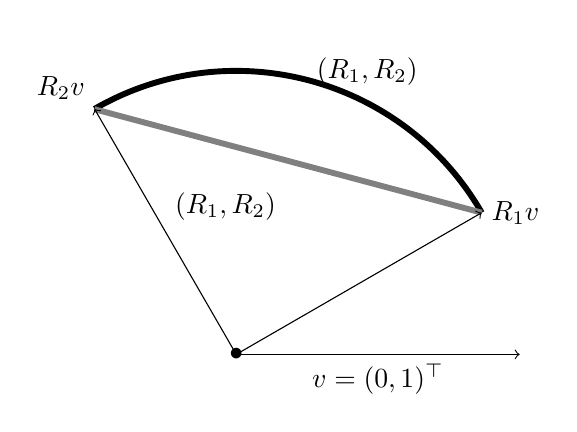
\begin{tikzpicture}[scale=.9]
%\draw (0,0) circle (4cm);
\draw (0,0) node {$\bullet$};
\draw (3.464102,2) node[anchor =  west]{$\bm R_1\bm v$};
\draw [->] (0,0)--(4,0);
%\draw [->] (4,0) arc (0:30:4cm);
\draw (2,0) node[anchor = north]{$\bm v=(0,1)^\top$};
\draw (-2,3.46) node[anchor = south east]{$\bm R_2\bm v$};
\draw [line width=.75mm] (3.464102,2) arc (30:120:4cm);
\draw[line width=.75mm, color=gray] (-2,3.46)--(3.464102,2);
\draw [->](0,0) -- (-2,3.464102);
\draw [->](0,0)--(3.464102,2);
\draw (1,3.66) node[anchor= south west]{$\Rdist (\bm R_1,\bm R_2)$};
\draw (-1,1.75) node[anchor= south west]{$\Edist (\bm R_1,\bm R_2)$};
%\draw (0,0) circle (4cm);
%\draw (0,0) node {$\bullet$};
%\draw (0,0)--(4,0) node[anchor =  west]{$o_1$};
%\draw (4,0) node[anchor =  west]{$\bm R_1$};
%\draw (0,0)--(-2,3.46) node[anchor = south east]{$o_2$};
%\draw (-2,3.46) node[anchor = south east]{$\bm R_2$};
%\draw[line width=.75mm] (4,0) arc (0:120:4cm);
%\draw[line width=.75mm, color=gray] (-2,3.46)--(4,0);
%\draw (0,0)--(2,3.46) node[anchor= south west]{$\alpha$};
%\draw (2,3.46) node[anchor= south west]{$\Rdist (\bm R_1,\bm R_2)$};
%\draw (-1.25,0.73) node[anchor= south west]{$\Edist (\bm R_1,\bm R_2)$};
%\draw (3/8,.7)[->] arc (60:120:.75cm);
%\draw (0,1.2) node {$\frac{\alpha}{2}$};
%\draw (0,2.8) node {$\frac{\beta}{2}$};
%\draw (2,0) node[anchor=north]{1};
\end{tikzpicture}
\end{center}
\vspace{-.25cm}
\caption{An illustration of the Euclidean and Riemannian distance metric, where to simplify the visualization, we use $SO(2)$ (rotations of points on the $\mathbb R^2$ unit circle) in place of $SO(3)$.  Here $\bm R_1$, $\bm R_2$ are $2\times2$ rotation matrices in $SO(2)$, where $\bm R_1\bm v$ and $\bm R_2\bm v$ are points on the $\mathbb R^2$ unit circle  after rotating $\bm v = (0,1)^{\top}$ by  $\bm R_1$ and $\bm R_2$, respectively.  $\Rdist (\bm R_1,\bm R_2)$ is displayed by the curved line (black), $\Edist (\bm R_1,\bm R_2)$ by the straight line (gray).}
\label{fig:dEvsdG} 
\end{figure}

